\chapter{Genome Sequencing}
\label{genome}

\begin{preamble}
\depend{howabout}
Sequencing of a complete human genome represents one of the greatest
scientific achievements of the century.
%
When the human genome project was first proposed in mid 1980's, the
technology available could only sequence couple of hundred bases at a
time.
%
After a few decades, the efforts led to the several major landmark
accomplishments.
%
In 1996, the DNA of the first living species (fruit fly) was sequenced. 
%
This was followed, in 2001, by the draft sequence of the human genome.
%
Finally in 2007, the full human genome diploid was sequenced.
%
Efficient parallel algorithms played a crucial role in all these
achievements.  In this chapter, we review the genome-sequencing
problem and discuss how the problem can be formulated as an
algorithmic one.

This chapter presents an overview of the genome sequencing problem and how it may be abstracted and solved as a string problem in computer science.
\end{preamble}


\begin{code}
% Here is a C comment
% If we didn't skip over this, we would be in trouble.
% Because it is also a latex comment.
fib n {
  if n < 2 {
    n
  }
  else {
    return fib (n-1) + fib (n-2)

}
\end{code}

\begin{code}[language = c]
% Here is a C comment
% If we didn't skip over this, we would be in trouble.
% Because it is also a latex comment.
fib n {
  if n < 2 {
    n
  }
  else {
    return fib (n-1) + fib (n-2)

}
\end{code}


\section{Genome Sequencing Problem}
\label{genome::prob}




\subsection{Background}

%% \begin{flushleft}
%%   \quad
%%   \begin{tabular}{r l}
%%     % \rule
%%     1996 & sequencing of first living species, \\
%%     2001 & draft sequence of the human Genome, \\
%%     2007 & full human Genome diploid sequence.\\
%%     % \bottomrule
%%   \end{tabular}
%% \end{flushleft}

\begin{gram}


As with many ``real world'' applications, defining precisely the
problem that models our application is interesting in itself.  
%
We
therefore start with the vague and not well-defined problem of
``sequencing the human genome'' and convert it into a precise
algorithmic problem.  
%
Our starting point is the ``shotgun method'' for
genome sequencing, which was the method used for sequencing the human
genome.
\end{gram}


\begin{definition}[Nucleotide]
A nucleotide is the basic building block of nucleic acid polymers such
as DNA and RNA. 
%
It is comprised of a number of components, which bind together to form
the double-helix.
%
The components include 
\begin{itemize}
\item a~\defn{nitrogenous base}, one of Adenine,
Cytosine, Guanine, Thymine (Uracil), 

\item a 5-carbon sugar molecule, and
\item one or more phosphate groups.
\end{itemize}
%
We distinguish between four kinds of nucleotides based on their
nitgogenous base and label them as \str{A} (Adenine), \str{C}
(Cytosine), \str{G} (Guanine), or \str{T} (Thymine).
\end{definition}

\begin{definition}[Nucleic Acid]
Nucleic acids are large molecules structured as linear chains of
nucleotides.  DNA and RNA are two important examples of nucleic acids.
\end{definition}

\begin{definition}[Human Genome]

The~\defn{human genome} is the full nucleic acid sequence for humans
consisting of nucleotide bases of A (Adenine), Cytosine (C),
Guanine (G), or Thymine (T).
%
It contains over $3$ billion~\defn{base pairs}, each of which consist
of two nucleotide bases bound by hydrogen bonds.
%
It can be written as a sequence or a string of bases consisting of the
letters, ``A'', ``C'', ``G'', and ``T''.
%
\end{definition}

\begin{remark}
The human-genome sequence, if printed as a book, would be
about as tall as the Washington Monument.
%
The human genome is present in each cell of the human body. 
%
It appears to have all the information needed by the cells in our
bodies and its deeper understanding will likely lead to insights into
the nature of life.
\end{remark}
%% \begin{checkpoint}
%% \begin{questionfr}
%% \points 10
%% \prompt What is the difference between a nucleoite and a nucleic acid?
%% \answer 
%% % A nucleic acid consists of many necleoutides.
%% \end{questionfr}

%% \begin{questionfr}
%% \points 10
%% \prompt How long is the human genome?
%% \answer Human genome consist of over 3 Billion base pairs.
%% \explain
%% \end{questionfr}


%% \end{checkpoint}



\subsection{Sequencing Methods}


\begin{teachask}
What makes genome sequencing hard?
\end{teachask}
%

\begin{gram}
The challenge in sequencing the genome is that there is currently
no way to read long strands with accuracy. 
%
Current DNA ``reading'' techniques are only capable of efficiently
reading relatively short strands, e.g., 10-1000 base pairs, compared
to the over three billion contained in the whole human genome.
%
Scientists therefore cut strands into shorter fragments, sequence
them, and then reassemble the sequenced fragments.
%
\end{gram}


\begin{gram}[Primer Walking]  
A technique called~\defn{primer walking} can be used to sequence
nucleic acid molecules up to 10,000 bases.  
%
The basic idea behind primer walking is to sequence a nucleic acid
from each end using special molecules called~\defn{primers} that can
be used to read the first 1000 bases or so.
%
The process is then repeated to ``walk'' the rest of the nucleic acid
by using most recently read part as a primer for the next part.
%
Since the process requires constructing primers and since it is
sequential, it is only effective for sequencing short molecules.
\end{gram}


%
%% \begin{teachask}
%% Can you think of a way to parallelize primer walking? 
%% \end{teachask}

\begin{gram}[Fragments]
To sequence a larger molecule, we can cut it into~\defn{fragments},
which can be achieved in a lab, and then use primer walking to sequence
each fragment.
%
Since each fragment can be sequenced independently in parallel, this
would allow us to parallelize the hard part of sequencing.
%
The problem though is that we don't know how to assemble them
together, because the cutting process destroys the order of the
fragments.
%
%% \begin{question}
%% The problem of putting together the pieces is a bit like solving a
%% jigsaw puzzle. But it is harder. Can you see why?  Can you think of a
%% way of turning this into a jigsaw puzzle that we can solve?
%% \end{question}
%
\end{gram}

\begin{note}
The approach of dividing the genome and sequencing each piece
independently is somewhat analogous to solving a jigsaw puzzle but
without knowing the complete picture.
%
It can be difficult and perhaps even impossible to solve such a
puzzle.
\end{note}

\begin{example}
When cut, the strand \texttt{cattaggagtat} might turn into,
\texttt{ag}, \texttt{gag}, \texttt{catt}, \texttt{tat}, destroying the
original ordering.
\end{example}

\begin{gram}[The Shotgun Method]
When we cut a genome into fragments we lose all the information
about how the fragments should be assembled.
%
If we had some additional information about how to assemble them, then
we could imagine solving this problem.
%
%\begin{question}
%Can you think of a way to relate different pieces? 
%\end{question}
One way to get additional information on assembling the fragments is
to make multiple copies of the original sequence and generate many
fragments that overlap.
%
Overlaps between fragments can then help relate and join them.
%
This is the idea behind the shotgun (sequencing) method, which was the
primary method used in sequencing the human genome for the first time.
\end{gram}

\begin{example}
For the sequence
%
\texttt{cattaggagtat}, 
%
we produce three copies:

\begin{quote}
\texttt{cattaggagtat}\\
\texttt{cattaggagtat}\\
\texttt{cattaggagtat}
\end{quote}

We then divide each into fragments
%
\begin{quote}
\texttt{catt}~~|~~\texttt{ag}~~|~~\texttt{gagtat}
\\
\texttt{cat}~~|~~\texttt{tagg}~~|~~\texttt{ag}~~|~~\texttt{tat}
\\
\texttt{ca}~~|~~\texttt{tta}~~|~~\texttt{gga}~~|~~\texttt{gtat}
\end{quote}
 
Note how each cut is ``covered'' by an overlapping fragment telling us
how to patch together the cut.

\end{example}

\begin{definition}[Shotgun Method]

The~\defn{shotgun method} works as follows.
\begin{enumerate}
\item Take a DNA sequence and make multiple copies.  

\item Randomly cut the sequences using a ``shotgun'' (in reality,
  using radiation or chemicals) into short fragments.

\item Sequence each fragments (possibly in parallel).

\item Reconstruct the original genome from the fragments.  
\end{enumerate}
\end{definition}

\begin{remark}
Steps 1--3 of the Shotgun Method are done in a wet lab, while step~4
is the algorithmically interesting component.
%
%\begin{question}
%In step 4, is it always possible to reconstruct the sequence?
%\end{question}
%
Unfortunately it is not always possible to reconstruct the exact
original genome in step~4. 
%
For example, we might get unlucky and cut all sequences in the same
location.  
%
Even if we cut them in different locations, there can be many DNA
sequences that lead to the same collection of fragments. 
%
A particularly challenging problem is repetition: there is no easy way
to know if repeated fragments are actual repetitions in the sequence
or if they are a product of the method itself.
%
\end{remark}
%% \begin{checkpoint}

%% \begin{questionfr}
%% \points 10
%% \prompt
%%  How large are the nucleic acids that can be ``read'' easily in
%% a lab today?
%% \answer
%% It is possible to read molecules up to 1000 nucleotides.
%% \end{questionfr}


%% \begin{questionfr}
%% \points 10
%% \prompt
%%  How large are the nucleic acids that can be ``read'' easily in
%% a lab today?
%% \answer
%% It is possible to read molecules up to 1000 nucleotides.
%% \end{questionfr}

%% \begin{questionfr}
%% \points 10
%% \prompt How does the primer walking technique work? 
%% \answer It works by sequencing a molecule in small chunks by starting
%% with a primer molecule that can be used to start reading the chunk. To
%% start the process, primers can be constructed.  Once the process
%% starts it can be iterated because the last chunk serves as a primer
%% for the next.
%% \explain
%% \end{questionfr}

%% \begin{questionfr}
%% \points 10
%% \prompt Is primer walking parallel?
%% \answer The technique is sequential because it requires a primer.
%% \explain
%% \end{questionfr}

%% \begin{questionfr}
%% \points 10
%% \prompt How does the shotgun method differ from primer walking?
%% \answer The difference is that in the shotgun method, we make copies
%% of the original molecule.  This allows us to assemble the results from
%% independent readings together.
%% \explain
%% \end{questionfr}


%% \end{checkpoint}

\subsection{Genome Sequencing Problem}

\begin{gram}
This section formulates the genome sequencing problem as an
algorithmic problem.
\end{gram}

\begin{gram}
Recall that the using the Shotgun Method, we can construct and sequence
short fragments made from copies of the original genome. 
%
Our goal is to use algorithms to reconstruct the original genome
sequence from the many fragments by somehow assembling back the
sequenced fragments.
%
But there are many ways that such fragments can be assembled and we
have no idea how the original genome looked like.  So what can we do?
%
In some sense we want to come up with the ``best solution'' that we
can, given the information that we have (the fragment sequences).
%
\end{gram}

\begin{gram}[Basic Terminology on Strings]
From an algorithmic perspective, we can treat a genome sequence just
as a sequence made up of the four different characters representing
nucleotides.
%
To study the problem algorithmically, let's review some basic
terminology on strings.
\end{gram}

%% TODO: Cleanup these definitions
%% You need substring first and then superstring.
\begin{flex}
\begin{definition}[Superstring]
A string $r$ is a~\defn{superstring} of another string $s$ if $s$
occurs in $r$ as a contiguous block, i.e., $s$ is a substring of $r$.
\end{definition}

\begin{example}
\begin{itemize}
\item
\texttt{tagg} is a superstring of \texttt{tag} and \texttt{gg} but not
of \texttt{tg}.

\item
\texttt{gtat} is a superstring of \texttt{gta} and \texttt{tat} but not
of \texttt{tac}.
 
\end{itemize}

\end{example}

\end{flex}

\begin{flex}
\begin{definition}[Substring, Prefix, Suffix]
A string $s$ is a~\defn{substring} of another string $r$, if $s$ occurs
in $r$ as a contiguous block.
%
A string $s$ is a~\defn{prefix} of another string $r$, if $s$ is a substring
starting at the beginning of $r$.
% 
A string $s$ is a~\defn{suffix} of another string $r$, if $s$ is a substring
ending at the end of $r$.
\end{definition}

\begin{example}
\begin{itemize}
\item
\texttt{ag} is a substring of \texttt{ggag}, and is also a suffix. 
\item
\texttt{gga} is a substring of \texttt{ggag}, and is also a prefix.
\item
\texttt{ag} is not a substring of \texttt{attg}.
\end{itemize}
\end{example}
\end{flex}

\begin{flex}
\begin{definition}[Kleene Operators]
For any set $\Sigma$, its~\defn{Kleene star} $\Sigma^*$ is the set of
all possible strings consisting of characters $\Sigma$, including the
empty string.

For any set $\Sigma$, its~\defn{Kleene plus} $\Sigma^+$ is the set of
all possible strings consisting of characters $\Sigma$, excluding the
empty string.
\end{definition}

\begin{example}
Given $\Sigma = \{\texttt{a},\texttt{b}\}$,
\[
\begin{array}{rl}
\Sigma^* 
%
= 
%
\{
&
\str{}, 
%
\\
&
\str{\texttt{a}}, \str{\texttt{b}}, 
%
\\
&
\str{\texttt{aa}}, \str{\texttt{ab}}, 
\str{\texttt{ba}}, \str{\texttt{bb}}, 
\\
%
&
\str{\texttt{aaa}}, \str{\texttt{aab}}, \str{\texttt{aba}},
\str{\texttt{abb}},
\\
& \str{\texttt{baa}}, \str{\texttt{bab}}, \str{\texttt{bba}}, \str{\texttt{bbb}},
\\
%
&
\ldots
\\
\} &
\end{array}
\]
%
and
%
\[
\begin{array}{rl}
\Sigma^+
%
= 
%
\{
&
\str{\texttt{a}}, \str{\texttt{b}}, 
\\
%
&
\str{\texttt{aa}}, \str{\texttt{ab}}, 
\str{\texttt{ba}}, \str{\texttt{bb}}, 
\\
%
&
\str{\texttt{aaa}}, \str{\texttt{aab}}, \str{\texttt{aba}}, \str{\texttt{abb}}, 
\\
&
\str{\texttt{baa}}, \str{\texttt{bab}}, \str{\texttt{bba}}, 
\str{\texttt{bbb}},
\\
%
& \ldots
\\
\} & 
\\
\end{array}
\]
\end{example}
\end{flex}

\begin{definition}[Shortest Superstring (SS) Problem]
  Given an alphabet set $\Sigma$ and a set of finite-length strings
  $A \subseteq \Sigma^*$, return a shortest string $r$ that contains every $x
  \in A$ as a substring of $r$.

%% In this definition the notation $\Sigma^*$, the ``Kleene star'', means
%% the set of all possible non-empty strings consisting of characters
%% $\Sigma$.
\end{definition}

\begin{gram}[Genome Sequencing as a String Problem] 
We can now try to understand the properties of the genome-sequencing
problem.
\end{gram}

\begin{flex}
\begin{exercise}[Properties of the Solution]
What is a property that the result sequence needs to have in relation
to the fragments sequenced in the Shotgun Method?
\end{exercise}

\begin{solution}
Because the fragments all come from the original genome, the result
should contain all of them.  In other words, the result is
a~\defn{superstring} of the fragments.
%
\end{solution}
\end{flex}

\begin{flex}
\begin{exercise}
There can be multiple superstrings for any given set of fragments.
%
Which superstrings are more likely to be the actual genome?
%
\end{exercise}

\begin{solution}
One possibly good solution is the shortest superstring. 
%
Because the Shotgun Method starts by making copies of the original
sequence, by insisting on the shortest superstring, we would make sure
that the duplicates would be eliminated.
%
More specifically, if the original sequence had no duplicated
fragments, then this approach would eliminate all the duplicates
created by the copies that we made in the beginning.
%
%
\end{solution}
\end{flex}

\begin{teachnote}
The claim above could probably be made more precise, perhaps with an
example.
\end{teachnote}



\begin{gram}
We can abstract the genome-sequencing problem as an instance of the
shortest superstring problem where $\Sigma = \{a, c, g, t\}$.
%
We have thus converted a vague problem, sequencing the genome, into a
concrete mathematical problem, the SS problem. 
%
\end{gram}

\begin{remark}
  One might wonder why the shortest superstring is the ``right  
  answer'' given that there could be many superstrings.  Selecting the  
  shortest is an instance of what is referred to as Occam's razor---i.e.,
  that the simplest explanation tends to be the right one. 
%
As we shall discuss more later, the SS problem is not exactly the
right abstraction for the application of sequencing the genome,
because it ignores some important practical factors.
%
One issue is that the genome can contain repeated sections that are 
much longer than the fragments.
In this case the shortest is not the right answer, but there is not
enough information in the fragments to determine the right answer
even given infinite computational power.
One needs to add input to fix this issue.
%
Another issue is that there can be errors in reading the short
strings.  This could make it impossible to find the correct or even
reasonable superstring.    Instead one needs to consider
approximate substrings.
%
Fortunately, the basic approach described here can be generalized to
deal with these issues.
\end{remark}
%% \begin{checkpoint}

%% \begin{questionfr}
%% \points 10

%% \prompt Let $s$ be a string of size $n$ in $\Sigma^+$, where $\Sigma =
%% \{a, c, g, t \}.$  Imagine cutting $s$ into fragments and constructing
%% the shortest superstring $r$ of these fragments.  How many possible
%% shortest superstrings are there?  
%% \answer
%% The shortest string is no longer that $n$... So we have  a sum...

%% \end{questionfr}

%% \begin{questionfr}
%% \points 10

%% \prompt
%% Let $s$ be a large string and consider the string $r = ss$, i.e., $r$~is
%% obtained by concatenating $s$ with itself.  Suppose that we apply the
%% Shotgun Method to $r$, can we construct it back?  

%% \answer
%% Seems unlikely. 
%% \explain

%% \end{questionfr}


%% \end{checkpoint}


\subsection{Understanding the Structure of the Problem}
\label{genome::prob::understanding}

\begin{gram}
Let's take a closer look at the problem to make some observations.
\end{gram}

\begin{gram}[Observation 1]
We can ignore a fragment that is a substring of another fragment,
because it doesn't contribute to the solution.
%
For example, if we have \texttt{gagtat}, \texttt{ag}, and \texttt{gt},
we can throw out \texttt{ag} and \texttt{gt}. 
\end{gram}

\begin{definition}[Snippets]
In genome sequencing problem, we refer to the fragments that are not
substrings of others as~\defn{snippets}.
\end{definition}

\begin{gram}[Observation 2: Ordering of the snippets]
Because no snippet is a substring of another, in the result
superstring, snippets cannot start at the same position.
%
Furthermore, if one starts after another, it must finish after the
other.  
%
This leads to our second observation: in any superstring, the start
positions of the snippets is a strict (total) order, which is the same
order as their finish positions.
%

This observation means that to compute the shortest superstring of the
snippets, it suffices to consider the permutations of snippets and
compute for each permutation the corresponding superstring.
\end{gram}


\begin{example}
In our example, we had the following fragments.

\begin{quote}
\texttt{catt}~~|~~\texttt{ag}~~|~~\texttt{gagtat}
\\
\texttt{cat}~~|~~\texttt{tagg}~~|~~\texttt{ag}~~|~~\texttt{tat}
\\
\texttt{ca}~~|~~\texttt{tta}~~|~~\texttt{gga}~~|~~\texttt{gtat}
\end{quote}

The snippets are now:
$S = \{$
%
\texttt{catt}, \texttt{gagtat}, \texttt{tagg},  \texttt{tta}, \texttt{gga}
%
$\}$

%\begin{equation*}
%  S = \Big\{\texttt{catt}, \texttt{gagtat}, \texttt{tagg},  \texttt{tta}, \text%tt{gga}\Big\}.
%\end{equation*}

The other fragments
%
$\{$
%
\texttt{cat}, \texttt{ag}, \texttt{tat},
\texttt{ca}, \texttt{gtat}
% 
$ \}$ are all contained within the snippets.

Consider a superstring such as \texttt{cattaggagtat}.  The starting
points for the snippets are: 
%
$0$ for \texttt{catt}, 
%
$2$ for \texttt{tta},
%
$3$ for \texttt{tagg},
%
$5$ for \texttt{gga}, and
%
$6$ for \texttt{gagtat}.
\end{example}

\begin{gram}[Shortest Superstring of a Permutation]
Our second observation says that a superstring corresponds to a
permutation.  This leads to the natural question of how to find the
shortest superstring for a given permutation.
%
The following theorem tells us how.
\end{gram}

\begin{flex}
\begin{theorem}[Shortest Superstring by Overlap Removal]   
Given any start ordering of the snippets $s_1,s_2, \ldots, s_n$,
removing the maximum overlap between each adjacent pair of snippets
$(s_i,s_{i+1})$ gives the shortest superstring of the snippets for
that start ordering.
\end{theorem}
\begin{proof}
The theorem can be proven by induction.  
%
The base case is true since it is clearly true for a single snippet.
%
Inductively, we assume it is true for the first $i$ snippets, i.e.,
that removing the maximum overlap between adjacent snippets among
these $i$ snippets yields the shortest superstring of $s_1, \ldots,
s_i$ starting in that order.  
%
We refer to this superstring as $r_i$.
%
We now prove that the theorem it is true for $i$ then it is true for
${i+1}$.
%
Consider adding the snippet $s_{i+1}$ after $r_i$, we know that
$s_{i+1}$ does not fully overlap with the previous snippet ($s_{i}$)
by the definition of snippets.
%
Therefore when we add it on using the maximum
overlap, the resulting string $r_{i+1}$ will be $r_i$ with some new characters
added to the end.  
%
The string $r_{i+1}$ is a superstring of $s_0, \ldots, s_{i+1}$
because it includes $r_i$, which by induction is a superstring of
$s_0, \ldots, s_{i}$, and because it includes $s_{i+1}$.
%
It is also be the shortest since $r_i$ is the shortest for $s_1,
\ldots s_i$ and a shorter string would not include $s_{i+1}$, because
we have already eliminated the maximum overlap between $s_{i+1}$ and
$r_i$.
\end{proof}


\end{flex}

\begin{example}
In our running example, consider the following start ordering
\begin{quote}
  \texttt{catt}\, \texttt{tta}\, \texttt{tagg}\,
  \texttt{gga}\, \texttt{gagtat}
\end{quote}
When the maximum overlaps are removed we obtain \texttt{cattaggagtat},
which is indeed the shortest superstring for the given start ordering.
In this case, it is also the overall shortest superstring.
\end{example}


\begin{definition}[Overlap]
\label{def:genome::prob::overlap}
Define the function $\cdvar{overlap}$ as a function that computes the
maximum overlap between two ordered snippets, i.e., 
\[
\cdvar{overlap}(s_i, s_j)
\]
denotes the \defn{maximum overlap}~for $s_i$ followed by $s_j$.
%

For example, for \texttt{tagg} and \texttt{gga}, $\cdvar{overlap}$~(\texttt{tagg}, \texttt{gga}) = 2.
\end{definition}



%% \begin{checkpoint}
%% \begin{questionfr}[Start positions of snippets]
%% \points 10
%% \prompt
%% Consider the set of snippets for a genome sequence, and let
%% $s$ be a superstring of the snippets, such that each
%% snippet is contained in the superstring as substring.  Prove than no
%% two snippets can start at the same position in $s$.  
%% \answer
%% \end{questionfr}

%% \begin{questionfr}[End positions of snippets]
%% \points 10
%% \prompt
%% Consider the set of snippets for a genome sequence, and let
%% $s$ be a superstring of the snippets, such that each
%% snippet is contained in the superstring as substring.  Prove than no
%% two snippets can end at the same position in $s$.  
%% \answer
%% \end{questionfr}

%% \begin{questionfr}[Substring Check]
%% \points 10
%% \prompt
%% Given a string $s$ of length $n$, and a string $t$ of
%% length $m$: design an algorithm that checks whether $s$ is a
%% substring of $t$, and analyze the work and span of your
%% algorithms.
%% \answer

%% %%
%% %% Answer: Start at every position in $t$ and check for overlap. 
%% %%  Work: $O(nm)$ Span: $log(m) + log(n)$. 
%% %%


%% \end{questionfr}


%% \end{checkpoint}


\section{Algorithms for Genome Sequencing}
\label{genome::alg}

\begin{gram}[Overview]
In this chapter, we review some of the algorithms behind the
sequencing of genome, and more specifically the shortest superstring (SS) problem.
%
The algorithms are derived by using consider three algorithm-design
techniques: brute-force, reduction, and greedy.
\end{gram}

%% \begin{flushleft}
%%   \quad
%%   \begin{tabular}{r l}
%%     % \rule
%%     1996 & sequencing of first living species, \\
%%     2001 & draft sequence of the human Genome, \\
%%     2007 & full human Genome diploid sequence.\\
%%     % \bottomrule
%%   \end{tabular}
%% \end{flushleft}

\subsection{Brute Force}
\label{genome::alg::bf}

\begin{gram}
Designing algorithms may appear to be an intimidating task, because it
may seem as though we would need brilliant ideas that come out of
nowhere. 
%
In reality, we design algorithms by starting with simple ideas based
on several well-known techniques and refine them until  the
desired result is reached.
%
Perhaps the simplest algorithm-design technique (and usually the least
effective) is brute-force---i.e., try all solutions and pick the best.
\end{gram}


\begin{gram}[Brute Force Algorithm 1]
As applied to the genome-sequencing problem, a brute-force technique
involves trying all candidate superstrings of the fragments and
selecting the shortest one.
%
Concretely, we can consider all strings $x \in \Sigma^*$, and for each
$x$ check if every fragment is a substring.
%
Although we won't describe how here, such a check can be performed
efficiently.
%
We then pick the shortest $x$ that is indeed a superstring of
all fragments.
%

The problem with this brute-force algorithm is that there are an
infinite number of strings in $\Sigma^*$ so we cannot check them all.
%
But, we don't need to: we only need to consider strings up to
the total length of the fragments~$m$, since we can easily construct a
superstring by concatenating all fragments. 
%
Since the length of such a string is $m$, the shortest superstring has
length at most $m$.
\end{gram}

\begin{note}
Unfortunately, there are still $|\Sigma|^m$ strings of length $m$;
this number is not infinite but still very large.  For the sequencing
the genome $\Sigma = 4$ and $m$ is in the order of billions, giving
something like $4^{1,000,000,000}$.  
%
There are only about $10^{80}
\approx 4^{130}$ atoms in the universe so there is no feasible way we
could apply the brute force method directly.  
%
In fact we can't even apply it to two strings each of length $100$.
\end{note}


\subsection{Brute Force Reloaded}
\label{genome::alg::bf-reloaded}

\begin{gram}
We will now design better algorithms by applying the observations from
the \href{genome::prob::understanding}{previous section}. 
%
Specifically, we now know that we can compute the shortest superstring
by finding the permutation that gives us the shortest superstring, and
removing overlaps.
%
Let's first design an algorithm for removing overlaps.
\end{gram}


\begin{algorithm}[Finding Overlap]
Consider two strings~$s$ and~$t$ in that order.
%
To find the overlap between $s$ and $t$ as
%
%\defref{genome-prob::overlap},
%
\href{def:genome::prob::overlap}{defined before},
%
 we can use the brute force-technique:
consider each suffix of~$s$ and check if it is a prefix of~$t$ and
select the longest such match.
%

% Guy : need to add description of reduce

The work of this algorithm is $O(|s| \cdot |t|)$, i.e., proportional to the product of
the lengths of the strings since for each suffix of $s$ we compare one to
one to each character of the prefix ot $t$.
%
The comparisons across all suffixes and all characters within a suffix can be done in parallel
in constant span.
We however need to check that all characters match within a suffix, and then find the longest suffix for
which this is true.    These can both be done with what is called a reduce operation, which 
``sums'' across a sequence of elements using a binary associative operator (in our case logical-and, and maximum).
If implemented using a tree sum, a reduce has span that is logarithmic in the input length.   Reduce will be covered
extensively in later chapters.
The total span is thus $O(\lg{|s|} + \lg{|t|}) = O(\lg{(|s|+|t|)} + \lg{(|s|+|t|)}) = O(\lg{(|s|+|t|)})$.
\end{algorithm}

%
%\begin{question}
%How can we compute the overlap between two strings?
%\end{question}
%
%
\begin{algorithm}[Finding the Shortest Permutation]
Using the above algorithm for finding overlaps, we can compute the
shortest superstring of a permutation by eliminating the overlaps
between successive strings in the permutation.
%
We can then find the permutation with the shortest superstring by
considering each permutation and selecting the permutation with the
shortest superstring.
%
Since we can consider each permutation independently of the others,
this algorithm reveals parallelism.

\end{algorithm}

\begin{algorithm}[Finding the Shortest Permutation (Improved)]
We can improve our algorithm for finding the shortest permutation by
using a technique known as~\defn{staging}.
%
Notice that our algorithm repeatedly computes the overlap between the
same snippets, because the permutations all belong to the same set of
snippets.
%
Since we only remove the overlap between successive snippets in a
permutation, there are only $O(n^2)$ pairs to consider.
%
We can thus stage work of the algorithm more carefully:

\begin{itemize}
\item First,  compute the overlaps between each pair of snippets and
  store them in a dictionary for quick lookup.
\item Second, try all permutations and compute the shortest
  superstring by removing overlaps as defined by the dictionary.
\end{itemize}
%
\end{algorithm}

\begin{note}
Staging technique is inherently sequential: it creates a sequential
dependency between the different stages of work that must be done.  
%
If, however, the number of stages is small (in our example, we have
two), then this is harmless. 
\end{note}

\begin{gram}[Cost Analysis]
%
Let's analyze the work and the span of our staged algorithm.
%
For the analysis, let $W_1$ and $S_1$ be the work and span for the
first phase of the algorithm, i.e., for calculating all pairs of
overlaps in our set of input snippets $s = \{s_1, \ldots, s_n \}$.
%
Let $m = \sum_{x \in S} |x|$.
%
Using our algorithm, $\cdvar{overlap}(x,y)$ for finding the maximum overlap
between two strings $x$ and $y$, we have
\[
\begin{array}{lll}
W_{1} & \leq & \sum_{i=1}^{n}\sum_{j=1}^{n} W(\cdvar{overlap}(s_i,s_j)))\\
  & = & \sum_{i=1}^{n}\sum_{j=1}^{n} O(|s_i| |s_j|)\\
  & \leq & \sum_{i=1}^{n}\sum_{j=1}^{n} (c_1 + c_2 |s_i| |s_j|)\\
  & =    & c_1 n^2 + c_2 \sum_{i=1}^{n}\sum_{j=1}^{n} (|s_i| |s_j|)\\
  & =    & c_1 n^2 + c_2 \sum_{i=1}^{n} \left(|s_i| \sum_{j=1}^{n} |s_j|\right)\\
  & =    & c_1 n^2 + c_2 \sum_{i=1}^{n} (|s_i| m) \\
  & =    & c_1 n^2 + c_2 m \sum_{i=1}^{n} |s_i| \\
  & =    & c_1 n^2 + c_2 m^2\\
  & \in  & O(m^2)  ~~~~~~~~~~~~~~\mbox{since } m \geq n.
\end{array}
\]

Since all pairs can be considered in parallel, we have for span
\[
\begin{array}{lll}
S_{1} & \leq & \max_{i=1}^{n}\max_{j=1}^{n} S(\cdvar{overlap}(s_i,s_j)))
\\
S_{1} & \leq & \max_{i=1}^{n}\max_{j=1}^{n} O(\lg{(|s_i| + |s_j|)})
\\
     & \in  & O(\lg m).
\end{array}
\]
%
We therefore conclude that the first stage of the algorithm requires
$O(m^2)$ work and $O(\lg{m})$ span.

Moving onto the second stage, we want to compute the shortest
superstring for each permutation.
%
Given a permutation, we know that all we have to do is remove the
overlaps.
%
Since there are $n$ overlaps to be considered and summed, this
requires $O(n)$ work, assuming that we can lookup the overlaps in
constant time.
%
Since we can lookup the overlaps in parallel, the span is constant for
finding the overlaps and $O(\lg{n})$ for summing them, again using a reduce.
%
Therefore the cost for handling each permutation is $O(n)$ work and
$O(\lg{n})$ span.
%


Unfortunately, there are $n!$ permutations to consider.
%
In fact this is another form of brute-force in which we try all
possible permutations instead of all possible superstrings.
%
Even though we have designed reasonably efficient algorithms for
computing the overlaps and the shortest superstring for each
permutation, there are too many permutations for this algorithm to be
efficient.
%
For $n = 10$ strings the algorithm is probably feasible, which is
better than our previous brute-force algorithm, which did not even
work for $n = 2$.
%
However for $n = 100$, we'll need to consider
$100!  \approx 10^{158}$ combinations, which is still more than the
number of atoms in the universe. 
%
Thus, the algorithm is still not feasible if the number of snippets is
more than a couple dozen.
\end{gram}


\begin{teachnote}
Since all pairs can be computed in parallel seem to require pfor.
\end{teachnote}

% Guy -- this needs to be made more precise
%  I think it is Stirling not Sterling
% ~ means asymptotically equal, which is not how it is used

% \begin{note}
% Recall Sterling's approximation:
% \[
% n! \sim {\sqrt {2\pi n}}\left({\frac {n}{e}}\right)^{n}.
% \]
% Even more roughly, you can think of this as 
% \[
% n! \sim \left( {\frac {n}{2.56}}\right)^{n} \sim \left( {\frac {n}{2}}\right)^{n}\]

% The intuition is this: you have $n/2$ pairs multiplied all of which
% add up to $n+1$.  The largest of such pairs occur in the middle,
% i.e. when they are the same, so if all pairs were to be maximum, we
% would have $((n/2)^2)^{n/2} = (n/2)^n$.  Now they are not all equal to
% the maximum but many are close, because many of the numbers are close
% to middle $n/2,$ thus we get something roughly but less than $(n/2)^n$.
% \end{note}

%
\begin{remark}
The technique of staging used above is a key technique in algorithm
design and engineering.
%
The basic idea is to identify a computation that is repeated many
times and pre-compute it, storing it in a data structure for fast
retrieval.
%
Later instances of that computation can then be recalled via lookup
instead of re-computing every time it is needed. 
\end{remark}

%% \begin{checkpoint}

%% \begin{questionfr}[String concatenation]
%% \points 10
%% \prompt
%%   You are given a set of strings $s_1, \ldots, s_n$ and a target
%%   string $t$.

%% Use the brute-force technique to come up with an algorithm that
%% gives you a subset of the strings and the specific order in which they
%% can be concatenated to obtain the target string.
%% %
%% Analyze the work and spane of your algorithm.

%% \answer
%% \explain
%% \end{questionfr}


%% \begin{questionfr}[Compact String concatenation]
%% \points 10
%% \prompt
%% You are given a set of strings $s_1, \ldots, s_n$ and
%% another target string $t$.  
%% %
%% Use the brute-force technique to design an algorithm that gives you a
%% subset of the strings and the specific order in which they can be
%% concatenated while removing overlaps to obtain the target string.  For
%% example if you concatenate "parallel" and "elision", you will get
%% "parallelision".  Analyze the work and the span of your algorithm.

%% \answer
%% \explain
%% \end{questionfr}

%% \begin{questionfr}[Improved Overlap Finding]
%% \points 10
%% \prompt
%% Recall that we have used a brute-force algorithm for finding the
%% overlap between two strings. Can you improve on this algorithm? 

%% \answer
%% %% It should be possible.  Have not thought about it carefully.
%% \explain
%% \end{questionfr}


%% \end{checkpoint}


\subsection{Shortest Superstrings by Algorithmic Reduction}
\label{genome::alg::reduction-tsp}

\begin{gram}
Another fundamental technique in algorithm design is to reduce one
algorithms problem to another that has a known solution.
%
It is sometimes quite surprising that we can reduce a problem to
another, seemingly very different one.
%
Here, we will reduce the shortest superstring problem to the Traveling
Salesman Problem  (TSP), which might appear to be quite different.
\end{gram}

\subsection{Traveling Salesperson Problem}

\begin{gram}
The Traveling Salesperson Problem or TSP is a canonical 
problem dating back to the 1930s and has been extensively studied.
%
The two major variants of the problem are~\defn{symmetric} TSP
and~\defn{asymmetric} TSP, depending on whether the graph has
undirected or directed edges, respectively.
%
Both variants are known to be NP-hard, which indicates that it is
unlikely that they have an algorithm that has polynomial work.
%
One might ask why reduce the SS problem to a hard problem such as the
TSP problem.   Well it turns out that the SS problem is also NP-hard.    The
possible advantage of the reduction is that the TSP problem is such a
well studied problem that there are many reasonably effective
algorithms for the problem, even if not polynomial work.
\end{gram}

\begin{gram}
Asymmetric TSP requires finding a Hamiltonian cycle of the
graph such that the sum of the arc (directed edge) weights along the
cycle is the minimum of all such cycles.
%
A cycle is a path in a graph that starts and ends at the
same vertex and a~\defn{Hamiltonian cycle} is a cycle that visits
every vertex exactly once.
%
In general graphs might not have a hamiltonian cycle, and in fact it
is NP-hard to even check if a graph has such a cycle.    However, in
the TSP problem it is assumed that there is an edge between every
pair of vertices (this is called a \defn{complete graph}) 
and in this case a graph always has a hamiltonian cycle.
\end{gram}

\begin{example}[TSP Competition]
A poster from a contest run by Proctor and Gamble in 1962 is
reproduced below.  The goal was to solve a 33 city instance of the
TSP.  Gerald Thompson, a Carnegie Mellon professor, was one of the
winners.

\begin{center}
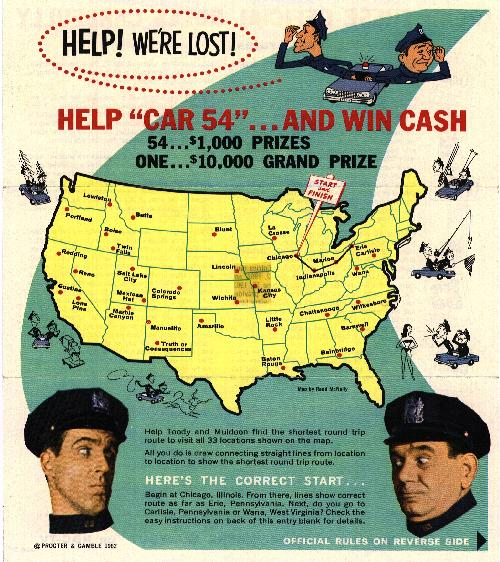
\includegraphics[width=4.0in]{genome/media/car54small.jpg}
\end{center}
\end{example}

\begin{problem}[The Asymmetric Traveling Salesperson Problem  (aTSP)]
  Given a weighted directed graph, find the shortest cycle that starts
  at some vertex and visits all vertices exactly once before returning
  to the starting vertex.
\end{problem}

\begin{gram}
The symmetric version of the problem considers undirected graphs
instead of directed ones---i.e., where the weight of an edge is the
same in both directions.
\end{gram}

\begin{note}
  Note that the version of the problem that requires starting at a
  particular vertex is also NP-hard because otherwise we can solve the
  general problem by trying each vertex.
\end{note}
%% \begin{question}
%% Can you reduce the SS problem to the TSP problem.  Hint: First try to
%% set up the problem so that each permutation corresponds to cycle.
%% \end{question}

\subsection{Reducing Shortest Superstrings to TSP}

\begin{gram}
We can reduce the Shortest Superstring problem to TSP by using 
our second Observation, which we also used in the brute-force
algorithm: the shortest superstring problem can be solved by trying
all permutations.
%
In particular we will make TSP try all the permutations for us.
%
\end{gram}


\begin{gram}[Reduction from SS to TSP]
For the reduction, we set up a graph so that each valid Hamiltonian cycle
corresponds to a permutation.  
%The graph is~\defn{complete}: it contains an arc between any two
%vertices, guaranteeing the existence of a Hamiltonian cycle.

%
We build a graph $D = (V, A)$.
%
The reduction relies on the overlap function defined
\href{def:genome::prob::overlap}{defined earlier}.

\begin{itemize}
\item The vertex set $V$ has one vertex per snippet and a special
  ``source'' vertex~$u$ where the cycle starts and ends.

\item The arc (directed edge) from $s_i $ to $s_j$ has weight $w_{i,j}
  = |s_j| - \cdvar{overlap}(s_i, s_j)$. 
%
 This quantity represents the increase
  in the string's length if $s_i$ is followed by $s_j$. 
%
  For example, if we have \texttt{tagg} followed by
  \texttt{gga}, then we can generate \texttt{tagga} which only
  adds 1 character giving a weight of 1---indeed,
  $|$ \texttt{gga}$|$ -
  $\cdvar{overlap}$ $($ \texttt{tagg}, \texttt{gga} $) = 3 -
  2 = 1$.

\item The weights for arcs incident to source $u$ are set as follows:
  $(u, s_i) = |s_i|$ and $(s_i, u) = 0$.  That is, if
  $s_i$ is the first string in the permutation, then the arc
  $(u, s_i)$ pays for the whole length $s_i$.  If $s_i$ is the
  last string we have already paid for it, so the arc $(s_i, u)$
  is free.
\end{itemize}
\end{gram}

\begin{example}
To see this reduction in action, the snippets in our running example,
%
\{\texttt{catt}, \texttt{gagtat}, \texttt{tagg},
  \texttt{tta}, \texttt{gga} \} 
%
results in the graph, a subgraph of which is shown below (not all arcs
are shown).

\begin{center}
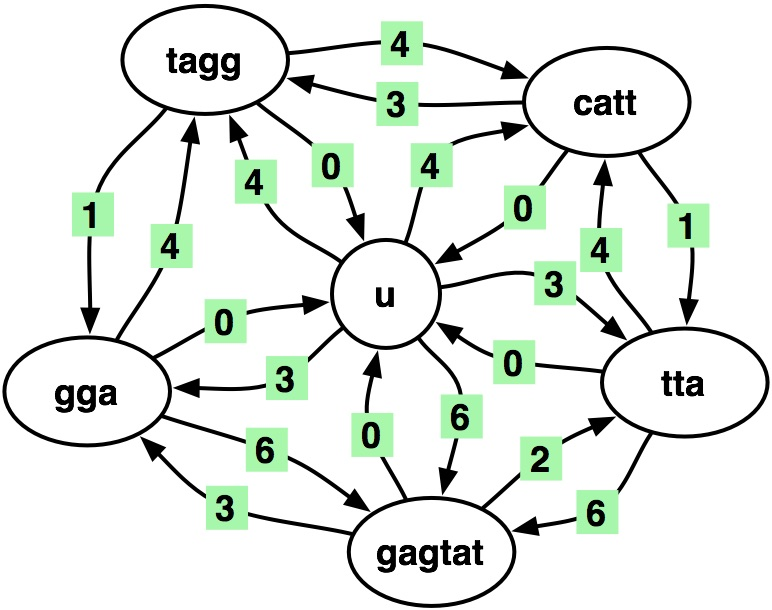
\includegraphics[width=3.0in]{genome/media/tsp-reduction.jpg}
\end{center}


%% \begin{question}
%%   What does a Hamiltonian cycle in the graph starting at the source
%%   correspond to? What about the total weight of the arcs on a cycle?
%% \end{question}

As intended, in this graph, a Hamiltonian cycle corresponds to
a permutation in our second brute-force method: we start from the source and
follow the cycle to produce the permutation.
%
Furthermore, the sum of the arc weights in that cycle is equal to the
length of the superstring produced by the permutation.
%
Since the TSP finds the minimum weight cycle, it also finds the
permutation that leads to the shortest superstring.
%
Therefore, if we could solve the TSP problem, we can solve the
shortest superstring problem.
%
\end{example}

\begin{gram}[Summary]
We have thus reduced the shortest-superstring problem, which is
NP-hard, to another NP-hard problem: TSP.
%
We constructed the reduction by using an insight from a brute-force
algorithm: that we can solve the problem by trying out all
permutations. 
%
The advantage of this reduction is that we know a lot about TSP, which
can help, because for any algorithm that solves or approximates TSP,
we obtain an algorithm for the shortest-superstring problem, and thus
for sequencing the genome.

\end{gram}

\begin{remark}[Hardness of Shortest Superstring]
In addition to designing algorithms, reductions can be used to prove
that a problem is NP-hard or NP-complete.  For example, if we reduce
an NP-hard (NP-complete) problem $A$ to another problem $B$ by
performing polynomial work, and preserving the size within a
polynomial factor, then $B$ must be NP-hard (NP-complete).

For example lets say we know the SS problem is NP hard.   Since we are
able to reduce it to the TSP problem in polynomial work and size using the
method described above, this tells us the TSP must be NP-hard.     If
we wanted to go the other way and prove SS is NP-hard based on the
known hardness of TSP then we would have to construct a reduction in the
other direction---i.e., from the TSP to the SS.      This is more
challenging and we will leave it up to the most motivated students.
\end{remark}

\begin{teachnote}
The reduction above has to try all sources.  It is actually reducing
to the TSP with start problem.
\end{teachnote}

%% \begin{checkpoint}
%% \begin{questionfr}[Hamiltonian cycle with start]
%% \points 10
%% \prompt

%% Prove using the reduction technique that if the TSP problem in
%% NP-hard, then so is the problem of finding the shortest Hamiltonian
%% cycle that starts and ends at a specified vertex.

%% \answer
%% \explain
%% \end{questionfr}

%% \end{checkpoint}

\subsection{Greedy Algorithm}
\label{genome::alg::greedy}

\begin{gram}
We have thus far developed a brute-force algorithm for solving the
Shortest Supersting problem that requires exponential time and reduced
the problem to the Traveling Salesperson Problem (TSP), which is
NP-hard.
%
We also remarked that the Shortest Superstring problem in NP-hard.
%
Thus, we are still far away from a polynomial-work solution to the
problem and we are unlikely to find one.
%

When a problem is NP hard, it means that there are {\em instances} of
the problem that are difficult to solve exactly.  
%
NP-hardness doesn't rule out the possibility of algorithms that
quickly compute approximate solutions or even algorithms
that exactly solve many real world instances.
%
For example the type-checking problem for strongly typed languages
(e.g., the ML family of languages) is NP-hard but we use them all the
time, even on large programs.
\end{gram}

\begin{gram}
One interesting approach to overcoming difficult NP-hard problems is
to use approximation.
%
For the SS problem, we know efficient approximation
algorithms that are theoretically good: they guarantee that the length
of the superstring is within a constant factor of the optimal answer.
%
Furthermore, these algorithms tend to perform even better in practice
than the theoretical bounds suggest.
%
In the rest of this unit, we discuss such an algorithm.
\end{gram}

\begin{gram}[Greedy Algorithms]
To design an approximation algorithm we will use an iterative design
technique based on a \defn{greedy heuristic}.
%
When applying this design technique, we consider the current solution
at hand and make a \defn{greedy}, i.e., locally optimal decision to
reduce the size of the problem.
%
We then repeat the same process of making a locally optimal decision,
hoping that eventually these decisions lead us to a global optimum.
%
For example, a greedy algorithm for the TSP can visit the closest
unvisited city (the locally optimal decision), removing thus one city
from the problem.
%

Because greedy algorithms rely on a heuristic they may or may not
return an optimal solution.
%
%
Nevertheless, greedy algorithms are popular partly because they tend
to be simple and partly because they can perform quite well.
%
We note that, for a given problem there might be several greedy
algorithms that depend on what is considered to be locally optimal.
%
\end{gram}


\begin{gram}
The key step in designing a greedy algorithm is to decide the locally
optimal decision.
%
In the case of the SS problem, observe that we can minimize the length
of the superstring by maximizing the overlap among the snippets.
%
Thus, at each step of the algorithm, we can greedily pick a pair of
snippets with the largest overlap and join them by placing one
immediately after the other and removing the overlap.  
%
This can then be repeated until there is only one string left.
%
This is the basic idea behind the greedy algorithm below.
\end{gram}

\begin{gram}[Computing Joins]
Let's define the function $\cdvar{join}(x, y)$ as a function that
places $y$ after $x$ and removes the maximum overlap.
%

For example, 
\\
%
$\cdvar{join}$~(\texttt{tagg}, \texttt{gga})~=~\texttt{tagga}.
%
\end{gram}


\begin{algorithm}[Greedy Approximate SS]
\label{alg:genome::alg::greedySS}
\[
\begin{array}{l}
\cdvar{greedyApproxSS}~(S) = 
\\
~~~~\cd{if}~|S| = 1~\cd{then}
\\ 
~~~~~~~~\cd{return}~x \in S
\\
~~~~\cd{else}
\\
~~~~~~~~\cd{let}
\\
~~~~~~~~~~~~T = \cset{(\cdvar{overlap}(x, y), x, y) : x \in S, y \in S, x \neq
  y}
\\
~~~~~~~~~~~~(o_{xy}, x, y) = \cdvar{argmax}_{(z, \_, \_) \in T} ~z
\\
~~~~~~~~~~~~z = \cdvar{join} (x, y)
\\
~~~~~~~~~~~~S' = S \cup \{z\} \setminus \{x,y\}
\\
~~~~~~~~\cd{in}
\\
~~~~~~~~~~~~\cdvar{greedyApproxSS}~(S')
\\
~~~~~~~~\cd{end}
\end{array}
\] 


The pseudocode for the greedy algorithm is shown above.
%
Given a set of strings $S$, the $\cdvar{greedyApproxSS}$ algorithm
checks if the set has only $1$ element, and if so returns that element.
%
Otherwise it finds the pair of distinct strings $x$ and $y$ in $S$
that have the maximum overlap.  It does this by first calculating the
overlap for all pairs and then picking the one of these that has the
maximum overlap.
%

Note that $T$ is a set of triples each corresponding to an overlap and
the two strings that overlap.  The notation 
\[
\cdvar{argmax}_{(z, \_, \_) \in T} z
\]
is mathematical notation for selecting the element of $T$ that
maximizes the first element of the triple, which is the overlap.
%

After finding the pair $(x,y)$ with the maximum overlap, the
algorithm then replaces $x$ and $y$ with $z = \cdvar{join}(x,y)$
in $S$ to obtain the new set of snippets $S'$.
%
The new set $S'$ contains one element less than $S$.
%
The algorithm recursively repeats this process on this new set of
strings until there is only a single string left.  It thus terminates
after $|S|$ recursive calls.
\end{algorithm}



\begin{flex}
\begin{exercise}
Why is the algorithm greedy?
\end{exercise}

\begin{solution}
The algorithm is greedy because at every step it takes the pair of
strings that when joined will remove the greatest overlap, a locally
optimal decision.  Upon termination, the algorithm returns a single
string that contains all strings in the original set $S$.  However,
the superstring returned is not necessarily the shortest superstring.
\end{solution}
\end{flex}

%% \begin{todo}
%% 	In the picture there should be a directed arrow from "gga" to "gagtat" with weight 2?
%% \end{todo}

\begin{example}
Consider the snippets in our running example, \\
%
\Big\{
%
\texttt{catt}, \texttt{gagtat}, \texttt{tagg}, \texttt{tta},
\texttt{gga}
%
\Big\}.  
%
\\
The graph below illustrates the overlaps between different snippets.
An arc from vertex $u$ to $v$ is labeled with the size of the overlap
when $u$ is followed by $v$.
%
All arcs with weight $0$ are omitted for simplicity.
%
\begin{center}
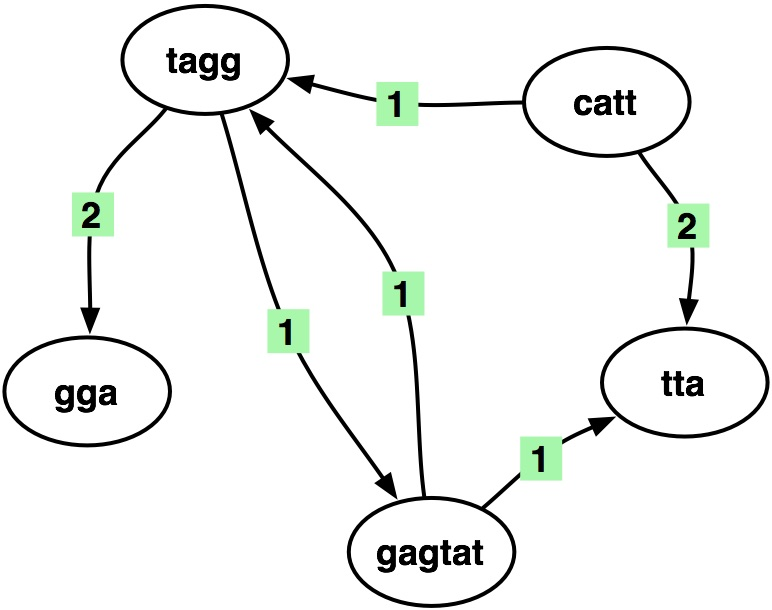
\includegraphics[width=3.0in]{genome/media/overlaps.jpg}
\end{center}

Given these overlaps, the greedy algorithm could proceed as follows:
\begin{itemize}
\item join \texttt{tagg} and \texttt{gga} to obtain \texttt{tagga}
  (overlap = 2),
\item join \texttt{catt} and \texttt{tta} to obtain \texttt{catta}
  (overlap = 2),
\item join \texttt{gagtat} and \texttt{tagga}  to obtain
  \texttt{gagtatagga} (overlap = 1), and
\item join \texttt{gagtatagga} and \texttt{catta} to obtain
  \texttt{gagtataggacatta} (overlap = 0).
\end{itemize} 

\end{example}

\begin{note}
Although the greedy algorithm merges pairs of strings one by one, we
note there is still significant parallelism in the algorithm, at least
as described.  In particular we can calculate all the overlaps in
parallel, and the largest overlap in parallel using a reduce.
\end{note}

\begin{gram}[Cost Analysis]
From the analysis of our brute-force algorithm, we know that we can
find the overlaps between the strings in $O(m^2)$ work and $O(\lg{m})$
span.
%
Thus $T$ can be computed in $O(m^2)$ work and $O(\lg{m})$ span.
%
Finding the maximum with $\cdvar{argmax}$ can be computed by a simple reduce operation.
%
Because $m > n$, the cost of computing $T$ dominates. 
%
Therefore, excluding the recursive
call, each call to $\cdvar{greedyApproxSS}$ costs is $O(m^2)$ work and
$O(\lg{m})$ span.
%%%%%

Observe now that each call to $\cdvar{greedyApproxSS}$ reduces the
number of snippets: $S'$ contains one fewer element than $S$, so
there are at most $n$ calls to $\cdvar{greedyApproxSS}$.  
%
These calls are sequential because one call must complete before the
next call can take place.  
%
Hence, the total cost for the algorithm is $O(n m^2)$ work and $O(n
\lg m)$ span.  
%
The algorithm therefore has parallelism (work over span) of $O(n m^2 / (n \lg m)) = O(m^2
/ \lg m)$ and is therefore highly parallel.
%
There are ways to make the algorithm more efficient, but leave that as
an exercise to the reader.
\end{gram}

\begin{gram}[Approximation Quality]
Since the $\cdvar{greedyApproxSS}$ algorithm does only polynomial work,
and since the TSP problem is NP hard, we cannot expect it to give an
exact answer on all inputs---that would imply \textbf{P} $=$
\textbf{NP}, which is unlikely.
%
Although $\cdvar{greedyApproxSS}$ does not return the shortest
superstring, it returns a good approximation of the shortest
superstring.
%
In particular, it is known that it returns a string that is within a
factor of 3.5 of the shortest; it is conjectured that the algorithm
returns a string that is within a factor of 2.  
%
In practice, the greedy algorithm typically performs better than the
bounds suggest.  The algorithm also generalizes to other similar
problems.
%
Algorithms such as $\cdvar{greedyApproxSS}$ that solve an NP-hard problem
to within a constant factor of optimal, are
called~\defn{constant-factor approximation algorithms}.
%
\end{gram}

%% \begin{checkpoint}
%% \begin{questionfr}[Contained Strings]
%% \points 10
%% \prompt
%%   In the greedy algorithm \cdvar{greedyApproxSS}
%% %  (\algref{genome::greedySS}), 
%% we remove ${x,y}$ from the set of strings but do not remove any
%% strings from $s$ that are contained within $xy = \cdvar{join}(x,y)$.
%% Prove that there cannot be any such strings.  
%% \answer 
%% \explain
%% \end{questionfr}


%% \begin{questionfr}[Correctness of the Greedy Algorithm]
%% \points 10
%% \prompt
%% Prove that algorithm $\cdvar{greedyApproxSS}$
%% % (\algref{genome::greedySS})
%% returns a string that is a superstring of all original strings.
%% \answer
%% \explain
%% \end{questionfr}

%% \begin{questionfr}[Exactness of Greedy Approximation]
%% \points 10
%% \prompt
%% Give an example input for which $\cdvar{greedyApproxSS}$
%% %(\algref{genome::greedySS}) 
%% does not return the shortest superstring.
%% \answer
%% \explain
%% \end{questionfr}


%% \begin{questionfr}[Improved Greedy Algorithm]
%% \points 10
%% \prompt
%% Improve the greedy algorithm's cost bounds by presenting a more
%% efficient implementation.
%% \answer
%% \explain
%% \end{questionfr}

%% \begin{questionfr}[Generous Grandmother]
%% \points 10
%% \prompt
%% Your rich grandmother enjoys collecting precious items, such as
%% jewelry and gold-plated souvenirs.  
%% %
%% When you visit her for Spring break (instead of going to Cancun), she
%% is very pleased and decides to reward you. She gives you a bag and a
%% scale and instructs you to take anything you want as long as the bag
%% does not hold any more than 10 pounds.  Delighted by the surprising
%% (based on your parents' stories of their childhood) generosity of your
%% grandmother, you also realize that your grandmother forgot to take the
%% price tags off the items, which gives you an idea about the value of
%% these items.


%% First, design a brute force algorithm for selecting the items to take
%% away with you. Is your algorithm optimal? What is the work and span of
%% your algorithm?

%% Next, design a greedy algorithm for selecting the items to take away
%% with you.  Why is your algorithm greedy?  Is your greedy algorithm
%% optimal? What is the work and span of your greedy algorithm?

%% \answer
%% \explain
%% \end{questionfr}

%% \end{checkpoint}

\section{Concluding Remarks}
\begin{gram}
The~\defn{Human Genome Project} was an international scientific
research project that was one of the largest collaborative projects in
the human history. 
%
The project was formally launched in 1990, after several years of
preparations, and pronounced complete in 2000.
%
It costed approximately three billion dollars (in the currency of
Fiscal Year 1991).

Abstracting a real-world problem such as the sequencing of the human
genome, which is one of the most challenging problems that has been
tackled in science, is significantly more complex than the relatively
simple abstractions that we  use in this book.  
%
This section discusses some of the complexities of genome sequencing
that we have not addressed.
\end{gram}

\begin{gram}[Abstraction versus Reality]
Often when abstracting a problem we can abstract away some key aspects
of the underlying application that we want to solve.  Indeed this is
the case when using the Shortest Superstring (SS) problem for
sequencing genomes.  In actual genome sequencing there are two
shortcomings with using the SS problem.
\end{gram}

\begin{gram}
The first is that when reading the base pairs using a DNA sequencer
there can be errors.  This means the overlaps on the strings that are
supposed to overlap perfectly might not.  This can be dealt with by
generalizing the Shortest Superstring problem to deal with approximate
matching.  Describing such a generalization is beyond the scope of
this course, but basically one can give a score to every overlap and
then pick the best one for each pair of fragments.  The nice feature
of this change is that the same algorithmic techniques we discussed
for the SS problem still work for this generalization, only the
``overlap'' scores will be different.
\end{gram}

\begin{gram}
The second shortcoming of using the SS problem by itself is that real
genomes have long repeated sections, possibly much longer than the
length of the fragments that are sequenced.  The SS problem does not
deal well with such repeats.  In fact when the SS problem is applied
to the fragments of an initial string with longer repeats than the
fragment sizes, the repeats or parts of them are removed.  One method
that researchers have used to deal with this problem is the so-called
\emph{double-barrel shotgun method}.  In this method strands of DNA
are cut randomly into lengths that are long enough to span the
repeated sections.  After cutting it up one can read just the two ends
of such a strand and also determine its length (approximately).  By
using the two ends and knowing how far apart they are it is possible
to build a ``scaffolding'' and recognize repeats.  This method can be
used in conjunction with the generalization of the SS discussed in the
previous paragraph.  In particular the SS method allowing for errors
can be used to generate strings up to the length of the repeats, and
the double barreled method can put them together.
\end{gram}

